
\documentclass[sigconf]{aamas}

\usepackage{listings}
\usepackage{float}
\usepackage{algorithm}
\usepackage{algorithmic}
\usepackage{soul}
\usepackage{amsmath}
\usepackage{wrapfig}

\setcopyright{ifaamas}
\acmConference[AAMAS '21]{Proc.\@ of the 20th International Conference on Autonomous Agents and Multiagent Systems (AAMAS 2021)}{May 3--7, 2021}{London, UK}{U.~Endriss, A.~Now\'{e}, F.~Dignum, A.~Lomuscio (eds.)}
\copyrightyear{2021}
\acmYear{2021}
\acmDOI{}
\acmPrice{}
\acmISBN{}

\title[AAMAS-2021 Formatting Instructions]{Auction-based Mechanisms for Resource-elastic Tasks\\in Edge Cloud Computing: Supplementary Material}

\begin{document}
\maketitle

% Section 1
\section{Server and task attributes of example problem case}
\label{sec:example-problem-case}
In Subsection 2.3, we present an example problem case to allow comparison with our flexible resource allocation and prior work's fixed resource allocation. Table~\ref{tab:example-server-properties} and~\ref{tab:example-task-properties} contains all of the server and task attributes respectively. Using this case, we show with graphical representations of server resource usage (figure 1 and 2), that the flexible resource allocation mechanism is able to respond to the servers limited resources by redistributing server resources. While for the fixed resource allocation mechanism, as it not able to redistributed resource causing it to not be able to run all of the tasks.

\begin{table}[h]
    \centering
    \caption{Table of task attributes. The columns ($s^{'}_j$, $w^{'}_j$, $r^{'}_j$) are fixed speeds which are not considered by the flexible resource allocation.}
    \label{tab:example-task-properties}
    \begin{tabular}{|c|c|c|c|c|c|c|c|c|}
        \hline
        Name    & $v_j$ & $s_j$ & $w_j$ & $r_j$ & $d_j$ & $s^{'}_j$ & $w^{'}_j$ & $r^{'}_j$ \\ \hline
        Task 1  & 100   & 100   & 100   & 50    & 10    & 24        & 30        & 20        \\ \hline
        Task 2  & 90    & 75    & 125   & 40    & 10    & 23        & 27        & 19        \\ \hline
        Task 3  & 110   & 125   & 110   & 45    & 10    & 35        & 28        & 18        \\ \hline
        Task 4  & 75    & 100   & 75    & 60    & 10    & 25        & 25        & 20        \\ \hline
        Task 5  & 125   & 85    & 90    & 55    & 10    & 21        & 27        & 21        \\ \hline
        Task 6  & 100   & 75    & 120   & 40    & 10    & 20        & 29        & 19        \\ \hline
        Task 7  & 80    & 125   & 100   & 50    & 10    & 33        & 28        & 19        \\ \hline
        Task 8  & 110   & 115   & 75    & 55    & 10    & 30        & 22        & 20        \\ \hline
        Task 9  & 120   & 100   & 110   & 60    & 10    & 30        & 28        & 22        \\ \hline
        Task 10 & 90    & 90    & 120   & 40    & 10    & 27        & 27        & 18        \\ \hline
        Task 11 & 100   & 110   & 90    & 45    & 10    & 25        & 27        & 20        \\ \hline
        Task 12 & 100   & 100   & 80    & 55    & 10    & 24        & 24        & 22        \\ \hline
    \end{tabular}
\end{table}

\begin{table}[h]
    \centering
    \caption{Table of server attributes}
    \label{tab:example-server-properties}
    \begin{tabular}{|c|c|c|c|}
        \hline
        Name     & $S_i$ & $W_i$ & $R_i$ \\ \hline
        Server 1 & 500   & 95    & 220   \\ \hline
        Server 2 & 500   & 95    & 210   \\ \hline
        Server 3 & 500   & 90    & 250   \\ \hline
    \end{tabular}
\end{table}

% Section 2
\section{Greedy algorithm pseudo-code}
In Subsection 3.1, we present the greedy algorithm based on prior work~\cite{sahni1975approximate} with a novel second stage to allow for the flexible resource allocation of the optimisation problem. The servers have the additional variables for the available storage, computation and bandwidth: $S^{'}_i$, $W^{'}_i$ and $R^{'}_i$ of server $i$.

\begin{algorithm}[h]
    \caption{Pseudo code of greedy algorithm}
    \label{alg:greedy-algorithm}
    \begin{algorithmic}
        \REQUIRE $J$ is the set of tasks and $I$ is the set of servers
        \REQUIRE $v(j)$ is the value density function of task $j$
        \REQUIRE $s(j, I)$ is the server selection function using task $j$ and set of servers $I$ returning the best server, or $\emptyset$ if the task is not able to be run on any server
        \REQUIRE $r(j, i)$ is the resource allocation function of a task $j$ and server $i$ returning the
            loading, compute and sending speeds
        \REQUIRE $\text{sort}(X, f)$ sorts a list of elements in descending order, based on a set $X$ with function, $f$ to compare elements

        \STATE{$J^{'} \leftarrow sort(J, v)$}
        \FORALL{$j \in J^{'}$}
            \STATE{$i \leftarrow s(j, I)$}
            \IF{$i \neq \emptyset$}
                \STATE{$s^{'}_j, w^{'}_j, r^{'}_j \leftarrow \gamma(j, i)$}
                \STATE{$x_{i,j} \leftarrow 1$}
            \ENDIF
        \ENDFOR
    \end{algorithmic}
\end{algorithm}

% Section 3
\section{Greedy algorithm solution to example problem case}
\begin{figure}[h]
    \centering
    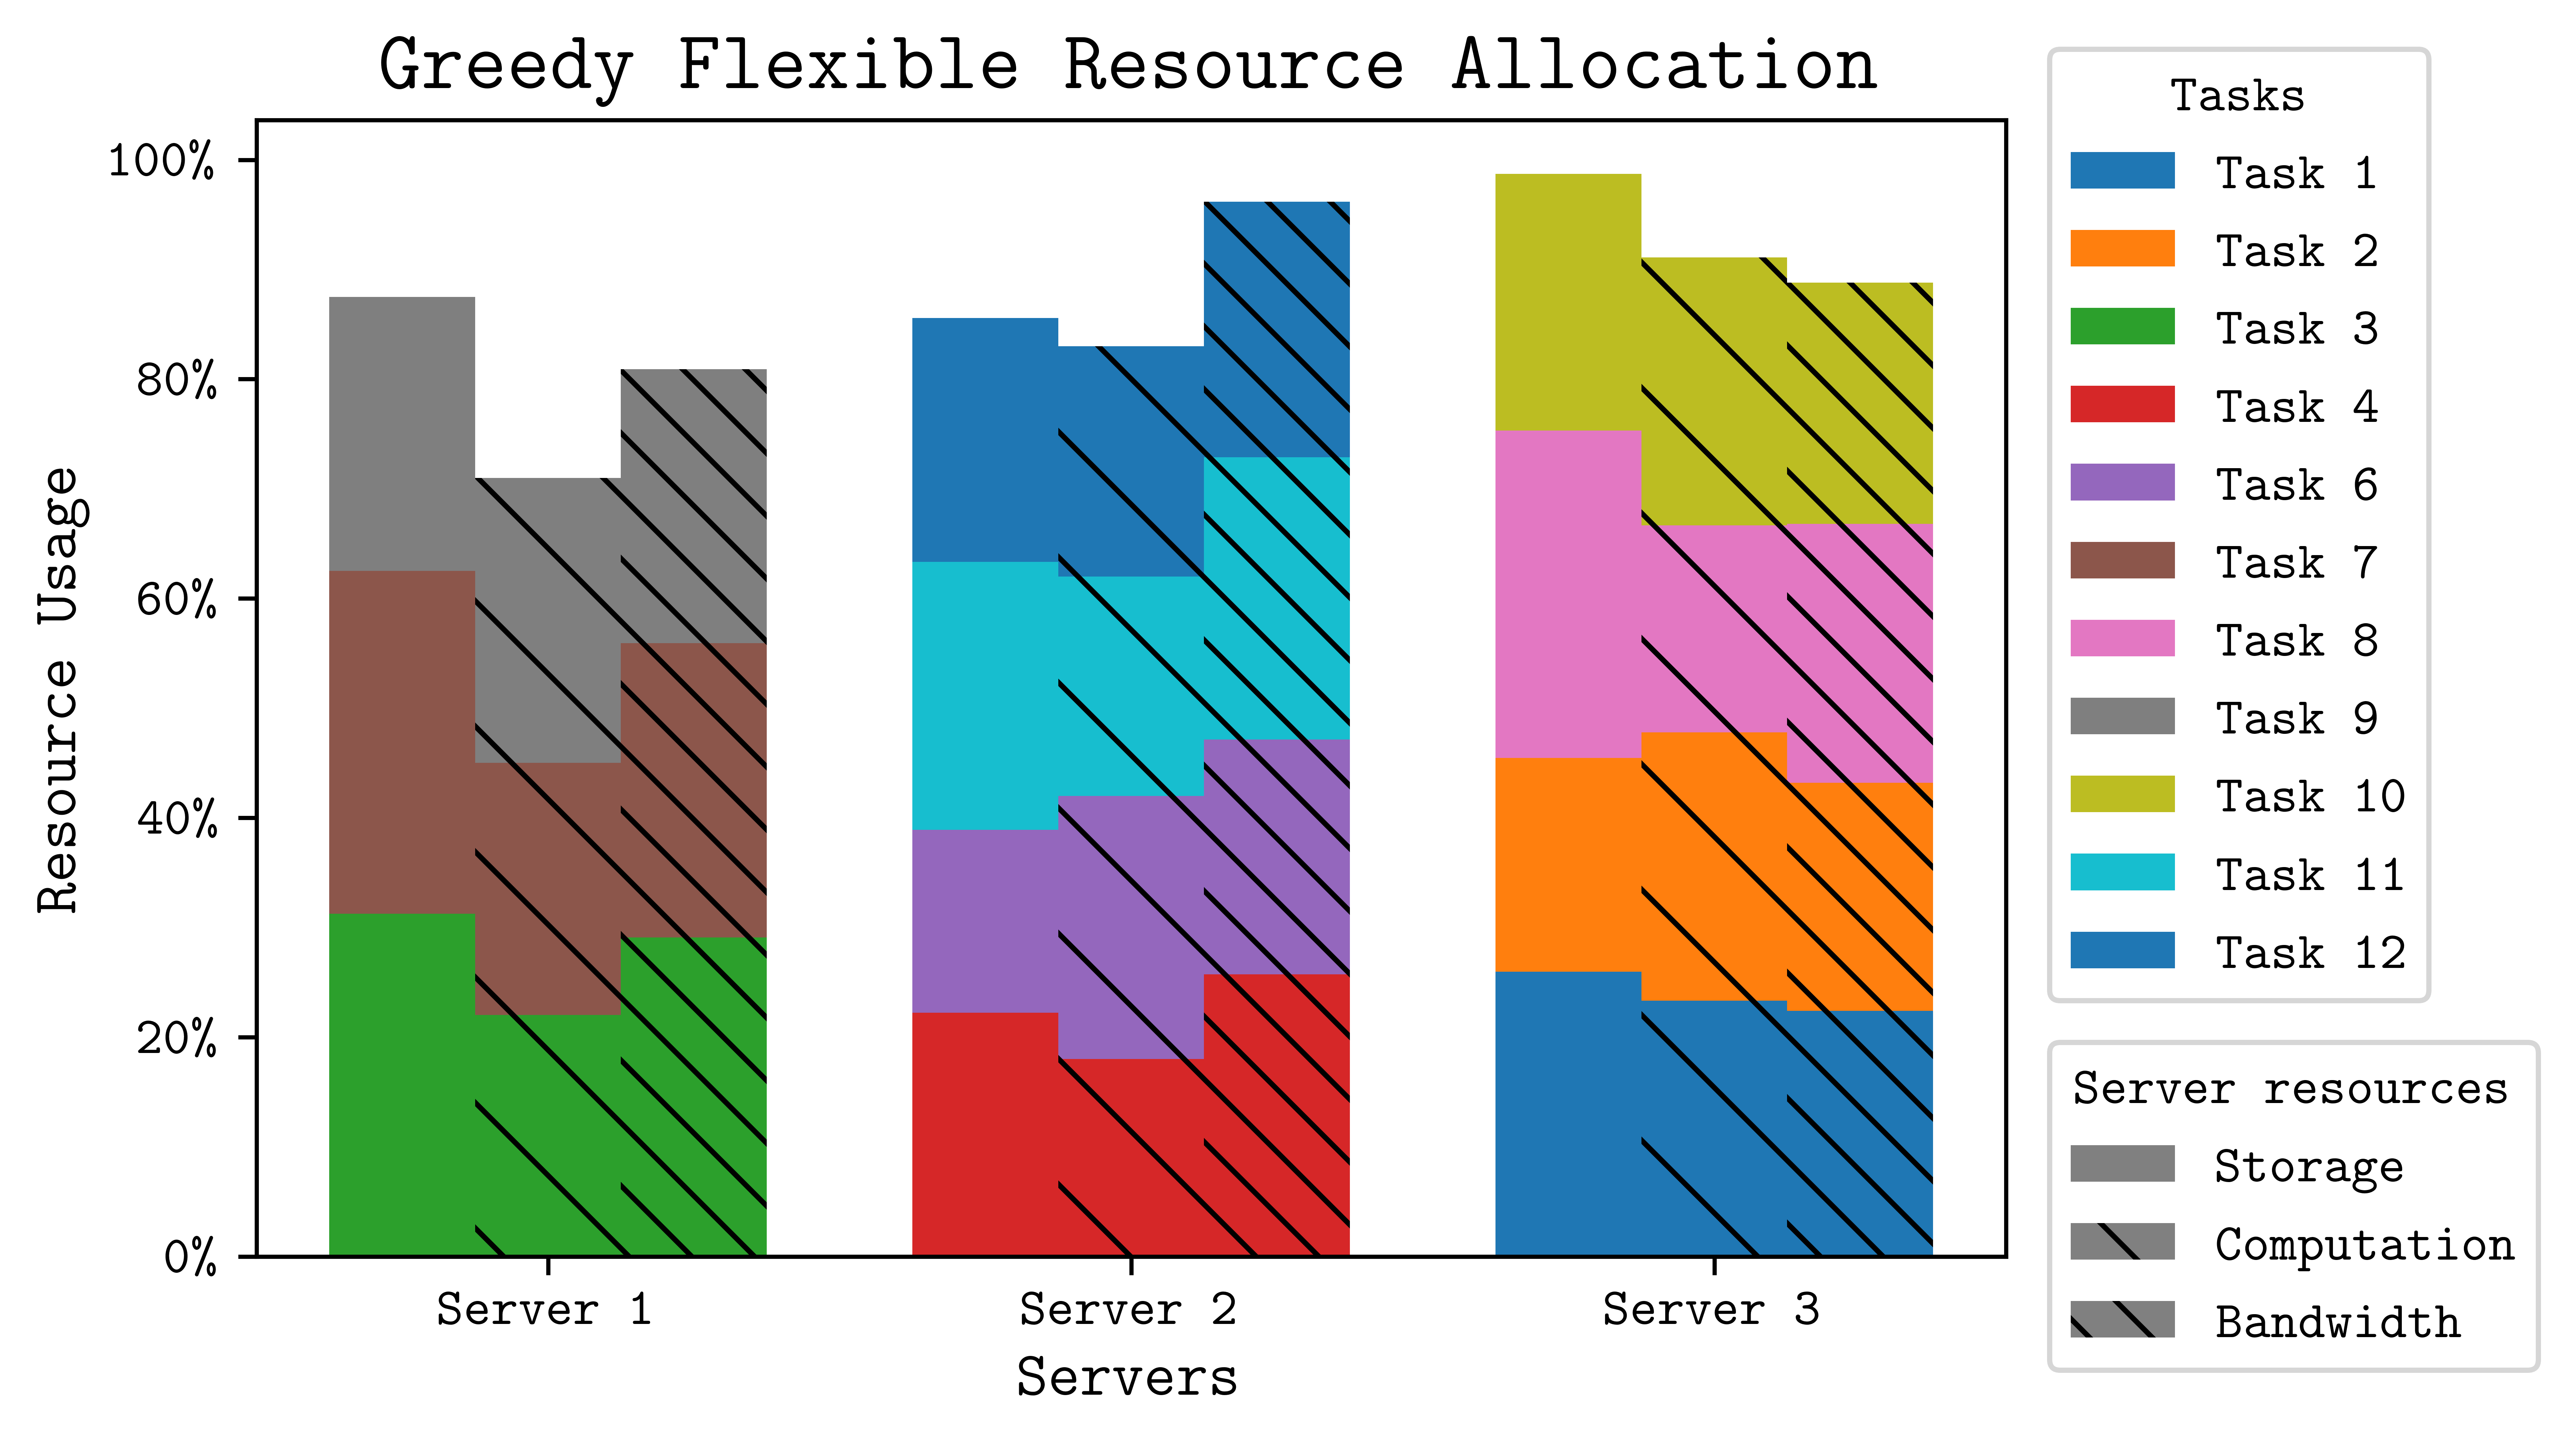
\includegraphics[width=\linewidth]{figs/allocation/greedy_flexible_resource_allocation.png}
    \caption{Example Greedy allocation using the model from section 1 with task and server attributes}
    \label{fig:example-greedy-allocation}
\end{figure}

In Section~\ref{sec:example-problem-case}, we present an example problem case to show the effectiveness of the flexible resource allocation mechanism over the fixed resource allocation mechanism. Figure~\ref{fig:example-greedy-allocation} is the solution to the example problem case using the greedy algorithm. Using the same modular function as in the evaluation of the greedy algorithm (Subsection 4.1), all of the tasks can be allocated. 

% Section 4
\section{Critical value auction pseudo-code}
In Subsection 3.2, we present the critical value auction based on Single Parameter Domain auctions (chapter 9.5.4)
of Algorithmic Game Theory~\cite{nisan2007algorithmic_cva}. 

\begin{algorithm}[h]
    \caption{Pseudo code of the Critical Value Auction}
    \label{alg:critical-value-auction}
    \begin{algorithmic}
        \REQUIRE $J$ is the set of tasks and $I$ is the set of servers
        \REQUIRE $S^{'}_i$, $W^{'}_i$ and $R^{'}_i$ is the available resources (storage, computation and bandwidth respectively) of server $i$
        \REQUIRE $v(j)$ is the value density function of task $j$
        \REQUIRE $v^{-1}(d, j)$ is the inverse of the value density function making the value the parameter of the function
        \REQUIRE $s(j, I)$ is the server selection function of task $j$ and set of servers $I$ returning the best server, or $\emptyset$ if the task is not able to be run on any server
        \REQUIRE $r(j, i)$ is the resource allocation function of a task and server returning a tuple of the loading, compute and sending speeds
        \REQUIRE $\text{sort}(X, f)$ is a function that returns a sorted list of elements in descending order, based on a set of elements $X$ and a function for comparing elements $f$
        \REQUIRE $\text{can\_allocate}(j, I)$ determines whether task $j$ can be allocated to any server $I$
        \REQUIRE $\text{greedy}(J, I, v, s, r)$ is the greedy algorithm (subsection 3.1) with tasks $J$, servers $I$, value density $v$, server selection policy $s$, resource allocation policy $r$.

        \STATE{$\text{greedy}(J, I, v, s, r)$}
        \FORALL{$j^{'} \in \{j \in J | \exists x_{j, i} \forall i \in I\}$}
            \FORALL{$j \in J$}
                \IF{$j^{'} \neq j$}
                    \STATE{$i \leftarrow s(j, I)$}
                    \IF{$i \neq \emptyset$}
                        \STATE{$s^{'}_j, w^{'}_j, r^{'}_j \leftarrow \gamma(j, i)$}
                    \ENDIF
                    \IF{$\neg \text{can\_allocate} (j^{'}, I)$}
                        \STATE{$p_{j^{'}} \leftarrow v^{-1}(v(j), j^{'})$}
                    \ENDIF
                \ENDIF
            \ENDFOR
        \ENDFOR
    \end{algorithmic}
\end{algorithm}

% Section 5
\section{Server relaxed optimisation problem}
As an upper bound, a server relaxed version of the optimisation problem (subsection 2.2) is used in Subsection 4.1. This differs from the original problem as a single "super" server exists where the resource capacity is equal to the sum of the servers resources. 

\begin{align}[h]
    \max & \sum_{\forall j \in J} v_j x_j \label{eq:relaxed-objective} \\
    \mbox{s.t.} \nonumber \\
    & \sum_{\forall j \in J} s_j x_j \leq S, \label{eq:relaxed-server-storage-constraint} \\
    & \sum_{\forall j \in J} w^{'}_j x_j \leq W,  \label{eq:relaxed-server-computation-constraint} \\
    & \sum_{\forall j \in J} (r^{'}_j + s^{'}_j) \cdot x_j \leq R \label{eq:relaxed-server-bandwidth-constraint} \\
    & \frac{s_j}{s^{'}_j} + \frac{w_j}{w^{'}_j} + \frac{r_j}{r^{'}_j} \leq d_j, &~ \forall{j \in J} \label{eq:relaxed-task-deadline} \\
    & 0 < s^{'}_j, &~ \forall{j \in J} \label{eq:relaxed-loading-speeds} \\
    & 0 < w^{'}_j, &~ \forall{j \in J} \label{eq:relaxed-compute-speeds} \\
    & 0 < r^{'}_j, &~ \forall{j \in J} \label{eq:relaxed-sending-speeds} \\
    & x_j \in \{0, 1\}, &~ \forall{j \in J} \label{eq:relaxed-task-allocation}
\end{align}

% Section 6
\section{Synthetic model}
For the evaluation of the work in Section 4, table~\ref{tab:synthetic-model-settings} contains the server and task attributes of the model used.

\begin{table}[h]
    \centering
    \caption{Table of task and server attribute mean and standard deviations (used in Section 4)}
    \label{tab:synthetic-model-settings}
    \begin{tabular}{|c|c|c|}
        \hline
        Attribute Name & Mean & Standard Deviation \\ \hline
        $v_j$          & 50   & 20                 \\ \hline
        $s_j$          & 100  & 15                 \\ \hline
        $w_j$          & 100  & 15                 \\ \hline
        $r_j$          & 50   & 10                 \\ \hline
        $d_j$          & 10   & 2                  \\ \hline
        $S_i$          & 450  & 50                 \\ \hline
        $W_i$          & 70   & 25                 \\ \hline
        $R_i$          & 290  & 45                 \\ \hline
    \end{tabular}
\end{table}

% Section 7
\section{Social welfare of auction mechanisms}
Figure~\ref{fig:auction-mechanims-social-welfare} shows the social welfare achieved by the auction mechanisms which is related to Section 4.2 that investigates the performances of the auction mechanisms.
\begin{figure*}[ht]
    \centering
    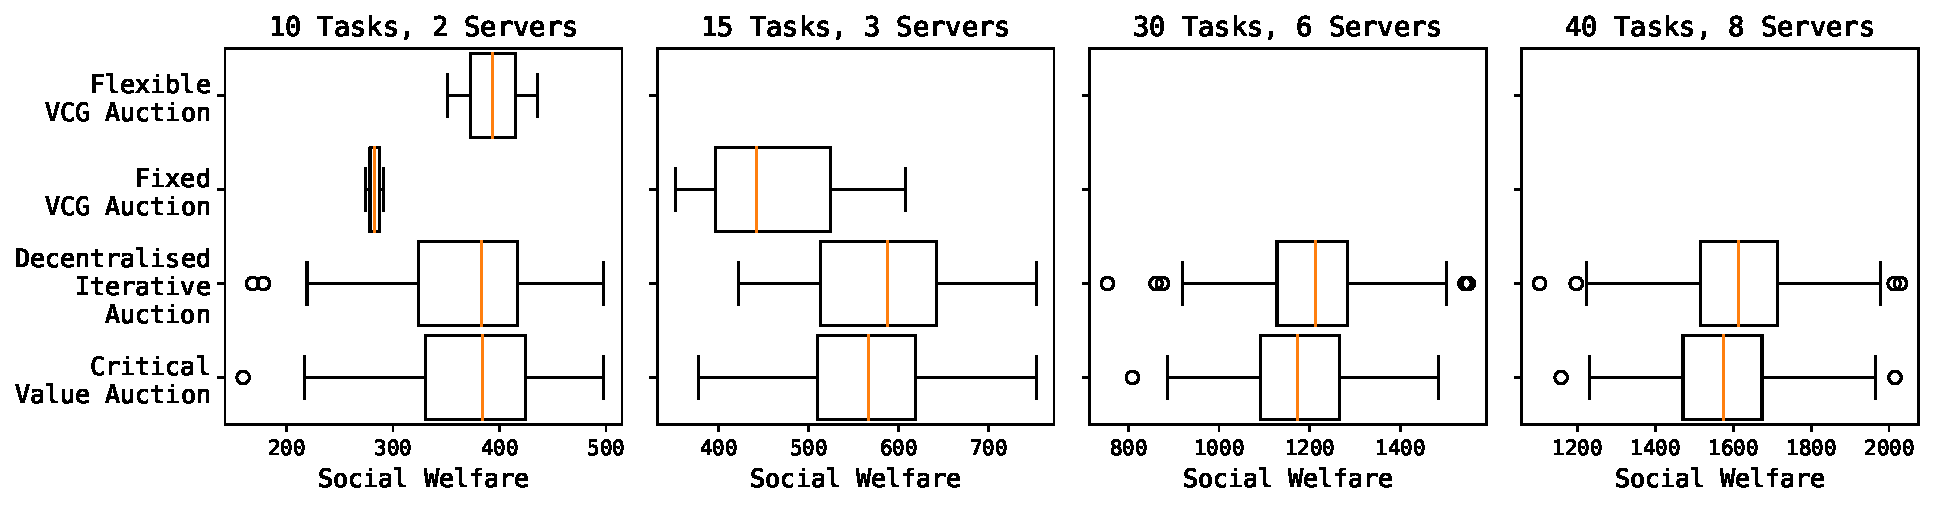
\includegraphics[width=\linewidth]{figs/auctions/social_welfare.pdf}
    \caption{Social welfare of the auction mechanisms: Flexible VCG auction, Fixed VCG auction, Critical Value Auction and Decentralised Iterative Auction.}
    \label{fig:auction-mechanims-social-welfare}
\end{figure*}

\bibliographystyle{ACM-Reference-Format} 
\bibliography{sections/references}

\end{document}